\section{Limits \& Continuity in 3D}
\noindent
Limits in single-variable calculus are relatively simple because thera are only two ways to approach a point on a curve: left and right. When dealing with a surface, there are infinitely many ways to approach a point. So, we need a general and more formal idea of limits that works in higher dimensions.

\subsection{Open Delta Neighborhoods}
\noindent
An open delta neighborhood of a point $x_0$ is defined as the set
\begin{equation*}
	N\left(x_0, \delta\right) = \left\{x \in \mathbb{R}^n \mid \norm{x-x_0} < \delta\right\}.
\end{equation*}

\begin{figure}[H]
	\centering
	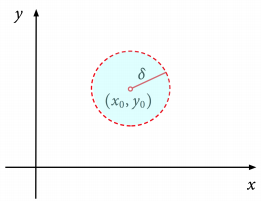
\includegraphics[width=0.5\textwidth]{./Images/differentialMultivariableCalculus/open_delta.png}
	\caption{An open delta neighborhood centered at $(x_0, y_0)$}
\end{figure}

\noindent
This simply means all points less than a distance $\delta$ away from point $x_0$.\\
For example, $N( (1,2) , 7) = \left\{ (x,y) \mid \sqrt{(x-1)^2 + (y-2)^2}<7 \right\}$, which is a ball (filled-in circle) of radius 7 centered at $(1, 2)$.
\subsection{Boundary Points, Open \& Closed Sets}
\noindent
Given some set $\Omega \subset \mathbb{R}^n$, $x$ is an interior point to $\Omega$ if $\exists \delta \mid N(x, \delta) \subset \Omega$. That is, $x$ is an interior point to $\Omega$ if you can draw a circle of non-zero radius around $x$ such that the entire circle is inside of $\Omega$.\\
All points that are not interior points are boundary points. Formally, $x$ is a boundary point of $\Omega$ if $\forall \delta \mid N(x,\delta) \not\subset \Omega$.\\
Using our definitions of interior and boundary points, we can define and open set as one that doesn't contain any of its boundary points and a closed set as one that contains all of its boundary point. Note that a set that contains some of its boundary points is neither open nor closed.
\subsection{Limit \& Continuity Definitions}
\noindent
Finally, we have the proper tools to define a limit in higher dimensions. We say that $\lim_{p\to p_0}f(p) = L$ if $\forall N(L\epsilon)$, $\exists N(p_0,\delta) \mid p \in N(p_0, \delta) \implies f(p) \in N(L, \epsilon)$.\\
That is, the limit of $f(p)$ as $p$ approaches $p_0$ is equal to $L$ if for all open delta neighborhoods around $L$, there exists an open delta neighborhood around $p_0$ such that $p$ being in the neighborhood around $p_0$ means $f(p)$ must be in the neighborhood around $L$.

[INSERT IMAGE]

\noindent
Now with a limit definition, we can define continuity at a point. We say that a function $f : \mathbb{R}^n \to \mathbb{R}$ is continuous at $p_0$ if $\lim_{p \to p_0}{f(p)} = f(p_0)$.\\

\noindent
\begin{theorem}
	Trigonometric functions, exponentials, logarithms, and sums, products, quotients, and compositions of such functions are continuous on their domain.
\end{theorem}

\noindent
Although our definitions allow us to confirm that a value is the limit of a function, they do not give us any insight into how to find the value of the limit. We'd need to approach our point of interest from every possible direction to see if the limit from that direction is the same as all the others. If any two directions give different limit values, then the limit doesn't exist.\\
We approach a function, $f$, by composing it with a single variable path, $\vec{r}(t)$, that goes through the point of interest, and find the limit along the path.\\

\noindent
If $f$ is some surface $f(x, y)$ and $\vec{r}(t) = \langle x(t), y(t)\rangle$, then the composition of $f$ and $\vec{r}$ is $f\circ\vec{r} = f(\vec{r}(t)) = f(x(t), y(t))$.\\
For example, let's try to find
\begin{equation*}
	\lim_{(x,y) \to (0,0)}{\frac{x^2-y^3}{x^2+y^2}}
\end{equation*}
\indent
We'll choose two paths $\vec{r_1}(t) = \langle t, 0 \rangle$ and $\vec{r_2}(t) = \langle t, t \rangle$ and find the limit as $t \to 0$ in both cases.\\
\indent
\begin{equation*}
	\lim_{t \to 0}{f(\vec{r_1}(t))} = \lim_{t \to 0}{\frac{t^2}{t^2}} = 1
\end{equation*}
\indent
\begin{equation*}
	\lim_{t \to 0}{f(\vec{r_2}(t))} = \lim{t \to 0}{\frac{t^2-t^3}{2t^2}} = \lim_{t \to 0}{\frac{1}{2} - \frac{t}{2}} = \frac{1}{2}
\end{equation*}
\indent
Since the limits on the two paths are not equal, we can say that
\begin{equation*}
	\lim_{(x,y) \to (0,0)}{\frac{x^2-y^3}{x^2+y^2}} = \text{ DNE}
\end{equation*}